\documentclass[a4paper,10pt]{article}
\usepackage[utf8]{inputenc}
\usepackage{graphicx}
\usepackage{gensymb}
\usepackage{textcomp}

%opening
\title{
  \begin{large}
    S \& S Assignment 6
  \end{large}
}
\author{R. Taarak\\ 17MCME14}

\begin{document}

\maketitle

\section{1. Write down as a difference equation with non-linearity; take a and c as 5 digit prime numbers and plot output for 1000 values.}
  \begin{figure}[!hbt]
    \centering
      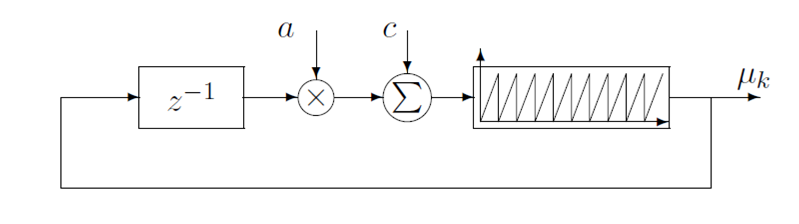
\includegraphics[scale=0.65]{image002.png}
    \caption{Linear congrential generator (LCG)}
  \end{figure}

  \Large{Sol:- }
  The non-linear function in the above block diagram is modulo function. 

\begin{itemize}
 \item First input is $\mu_k$.
 \item When it passes through \Large{$\bf{z^{-1}}$}, it becomes $\bf{\mu_{k-1}}$, further mulitiplied with 'a' becomes $\bf{a\mu_{k-1}}$.
 \item Further added with 'c' results in $\bf{a\mu_{k-1}+c}$.
 \item Now the new input to the modulo function is $\bf{a\mu_{k-1}+c}$. When it is passed through modulo function, the output is $\bf{(a\mu_{k-1}+c)\bmod n}$.
 \item Therefore, the difference equation is \[\bf{\mu_k = (a\mu_{k-1}+c)\bmod n}\] where 'a' and 'c' are 5 digit prime numbers and \[ k \in [0, 1000] \]
\end{itemize}

 \Large{\bf{Constraints on the values are: }}
\begin{itemize}
 \item $10000 < a < m$
 \item $10000 < c < m$
 \item $0 < \mu_{k-1} < m$
\end{itemize}

\Large{\bf{Data points:}}\\
\begin{center}
\begin{tabular}[!hbt]{| c | c |}
\hline
\centering
  \bf{x} & \bf{y} \\
  \hline
 1 & 0\\ 
 2 & 0\\  
 3 & 99997 \\
 4 & 79981 \\
 5 & 37828 \\
 6 & 99886 \\
 7 & 68509 \\
 8 & 24484 \\
 9 & 58666 \\
 10 & 80515 \\
 .. & .. \\
 .. & .. \\
 \hline
\end{tabular}
\end{center}

\begin{center}
 \begin{figure}[!hbt]
  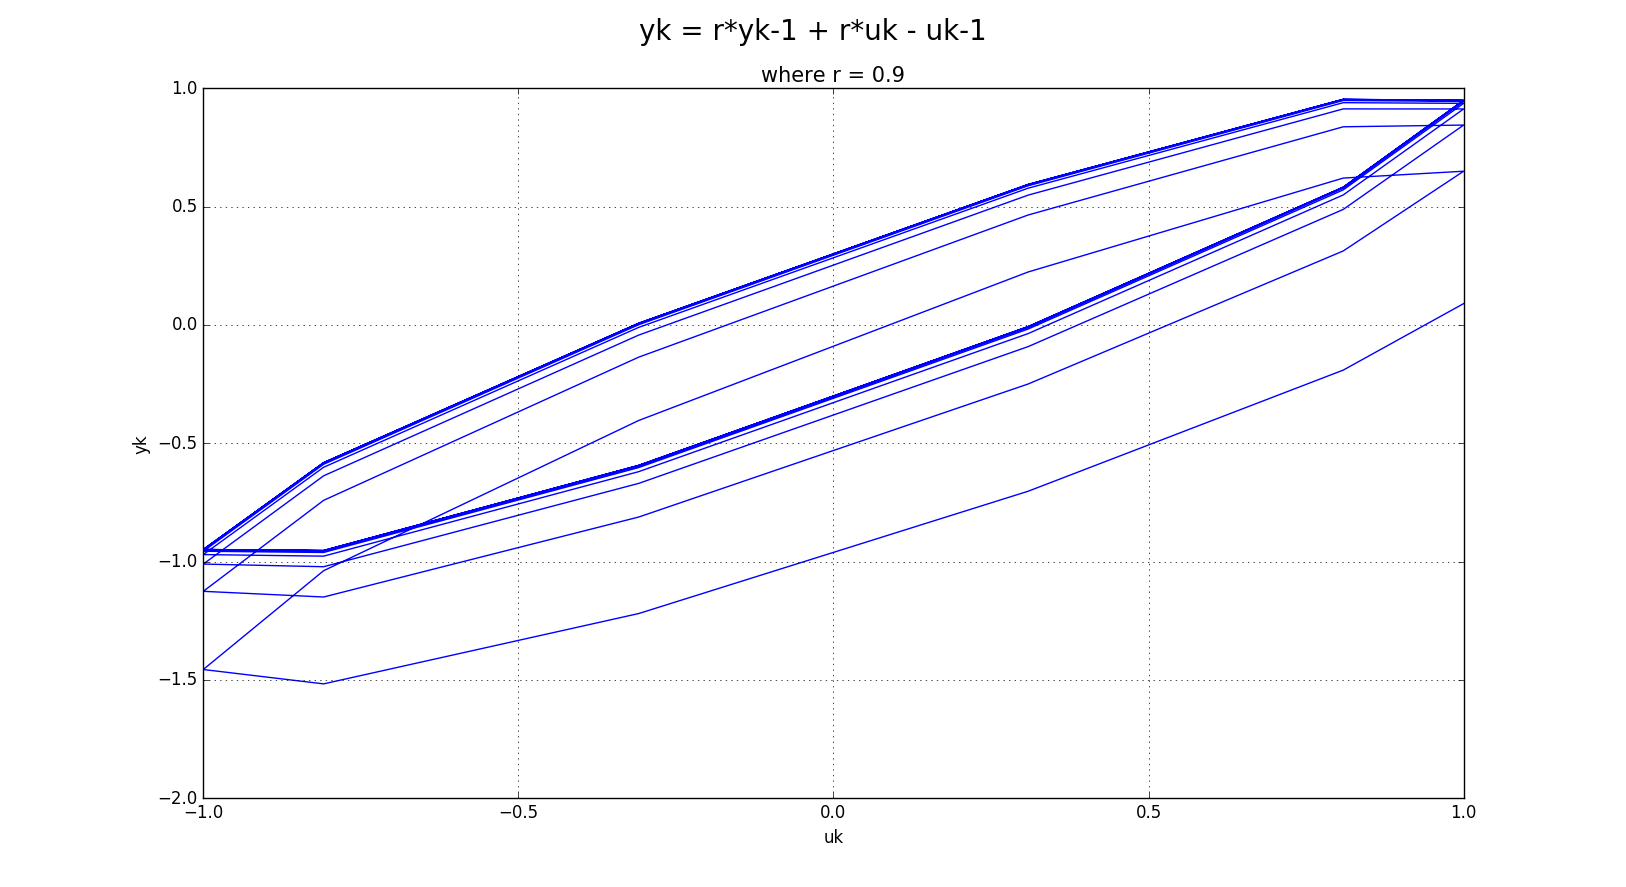
\includegraphics[scale=0.33]{figure_1.png}
 \end{figure}
\end{center}

\pagebreak
  \section{Use uk as cosine wave with f = 0.1, uk = (cos(2pifk) for 100 values get yk and  plot uk and yk for the below difference equation}
    $\bf{y_k = r.y_{k-1} + r.\mu_{k-1} - \mu_k}$
    
\begin{center}
\begin{tabular}[!hbt]{| c | c |}
\hline
  \bf{$u_k$} & \bf{$y_k$} \\
  \hline
 1.0 & 0.09\\ 
 0.809 & -0.19\\  
 0.309 & -0.702 \\
 -0.309 & -1.219 \\
 -0.809 & -1.516 \\
 -1.0 & -1.456 \\
 -0.809 & -1.038 \\
 -0.309 & -0.403 \\
 0.309 & 0.223 \\
 0.809 & 0.620 \\
 .. & .. \\
 .. & .. \\
 \hline
\end{tabular}
\end{center}

\begin{center}
 \begin{figure}[!hbt]
  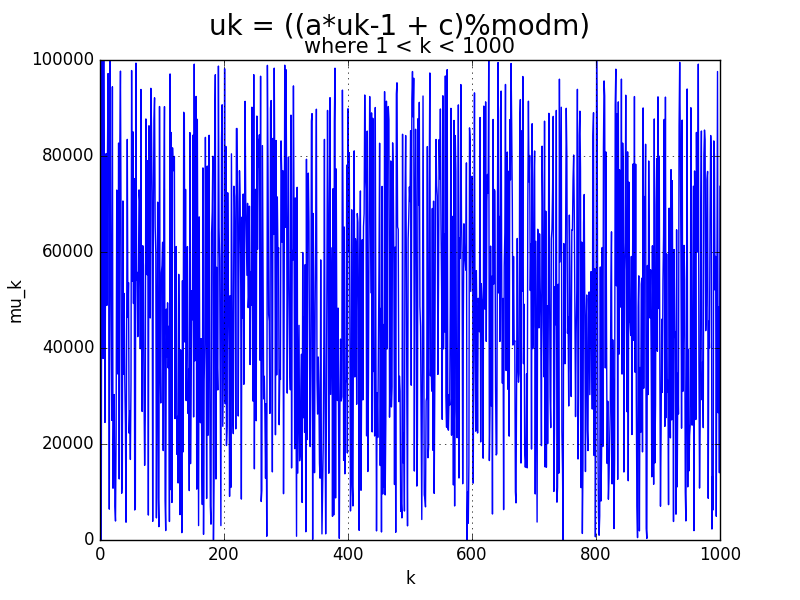
\includegraphics[scale=0.573]{figure_2.png}
 \end{figure}
\end{center}

\end{document}
